\newpage
% Sopaipillas
\begin{recipe}[source={Propia},
portion={10-15 porciones},
preparationtime={\unit[30]{Minutos}}
]{Sopaipillas sin zapallo}
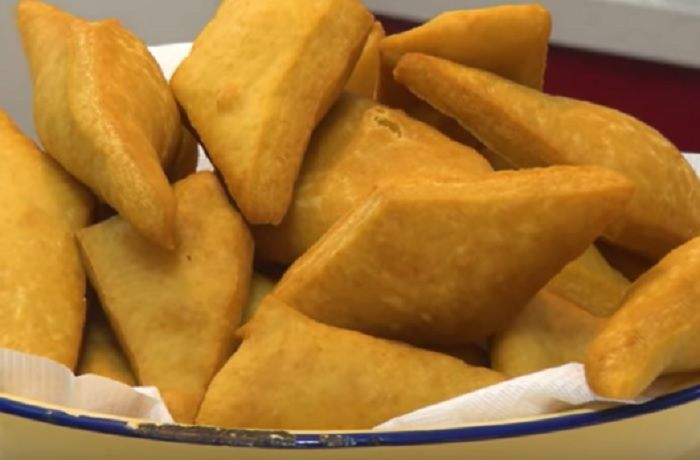
\includegraphics[width=0.25\textwidth]{Sopaipillas-sin-zapallo-surenas}
\introduction{
	Mi mami prepara unas sopaipillas muy ricas, pero modifiqué su receta y por eso es receta propia.
}
\ingredients{
	\underline{Para la masa} \\
	\unit[500]{gr} & de harina (2 tazones) \\
	\unit[15]{gr} & de levadura seca \\
	\unit[15]{gr} & de sal \\
	\unit[5]{gr} & de polvos de hornear \\
	\unit[5]{gr} & de bicarbonato \\
	\unit[350]{gr} & de agua a temperatura ambiente \\
	\underline{Para freir} \\
	\unit[50]{gr} & de manteca o \\
	\unit[$\frac{1}{2}$]{l} & de aceite
}
\preparation{
	\begin{enumerate}
		\item En un bol, integrar los ingredientes para realizar una masa y amasar hasta que la masa esté lista.
		\item Con un molde, o con un cuchillo, realizar los cortes deseados para las sopaipillas.
		\item En una sartén, poner a calentar el aceite o la manteca y esperar a que esté bien caliente.
		\item Freir las sopaipillas.
		\item Servir calentitas.
	\end{enumerate}
}
\hint{
	Se puede acompañar con pebre.
}
\end{recipe}